\documentclass[a4paper, 11pt, titlepage, twoside]{article}

\usepackage{preamble}

\begin{document}
%Canviem el nom de l'apartat Referències per ``Bibliografia''

%Portada

%%CANVIEU L'ESPAI VERTICAL ENTRE ELEMENTS SEGONS LA LLARGADA DEL TÍTOL
\begin{titlepage}
    {\centering
    {\Huge Master Thesis}\\
    \vspace{5mm}
    {\Large \textbf{Double MSc Degree in Industrial Engineering and Energy Engineering}}\\
    \vspace{20mm}
    \Huge \textbf{Dynamic Simulation and Stability Analysis of Power Systems: Development of RMS and EMT Tools within VeraGrid at eRoots}\\
    \vspace{10mm}
    \Large{January 2026}\\  %Data de la darrera complicació, si voleu posar una data fixa, escriviu-la aquí
    }
    \vspace{25mm}
    \hspace{2mm}
    \begin{tabular}{l@{ } l}
        \vspace{5mm}
        \Large \textbf{Author:} & \hspace{3mm} \Large{Maria Sans Esqué} \\
        \vspace{5mm}
    \Large\textbf{Supervisors:} & \hspace{3mm} \Large{Vinícius Albernaz Lacerda} \\
                                & \hspace{3mm} \Large{Josep Fanals i Batllori} \\

    \end{tabular}\par
    \vspace{10mm}
    {\centering
    \includegraphics[scale=0.3]{./Icones-ETSEIB-UPC/ETSEIB.png}\\
    {\Large Escola Tècnica Superior \\ d'Enginyeria Industrial de Barcelona}\\
    \vspace{3mm}
    \includegraphics[scale=0.4]{./Icones-ETSEIB-UPC/UPC.PNG}
    \par
    }
    \end{titlepage}

%Pàgina en blanc
\clearpage
\thispagestyle{empty}
\null\newpage 

%iniciem la numeració des del Resum
\pagenumbering{arabic}

\section*{Abstract}\label{Abstract}
\input{Chapters/Abstract}
\cleardoublepage
\section*{Resumen}\label{Resumen}
\input{Chapters/Resumen.tex}
\cleardoublepage
\section*{Resum}\label{Resum}
\input{Chapters/Resum.tex}

\cleardoublepage

\tableofcontents

\newpage
\listoffigures

\newpage
\begingroup
\setlength{\parskip}{0pt}
\listoftables %Opcional
\endgroup

\setlength{\abovedisplayskip}{5pt} % Equation spacing adjusted
\setlength{\belowdisplayskip}{5pt} % Equation spacing adjusted

\section*{Glossary}
\addcontentsline{toc}{section}{Glossary}
\subsection*{Symbols}
\begin{tabular}{l@{\hspace{1.95cm}} l}
  $\lambda$ & Eigenvalue \\
  $\zeta$ & Damping ratio \\
  $\bm{\omega}$ & Angular frequency vector \\
  $\bm{A}$ & State matrix \\
  $\bm{B}$ & Input matrix \\
  $\bm{C}$ & Output matrix \\
  $\bm{D}$ & Feedthrough matrix \\
  $\bm{x}$ & State vector \\
  $\bm{u}$ & Input vector \\
  $\bm{y}$ & Output vector \\
  $\tau$ & Time constant \\
  $V$ & Voltage module \\
  $\theta$ & Voltage angle\\
  $P$ & Active power\\
  $Q$ & Reactive power\\
  $g$ & Conductance\\
  $b$ & Susceptance\\
  $K_p$ & Proportional gain\\
  $M$ & Inertia constant\\
  $D$ & Damping coefficient\\
  $f$ & System frequency\\
  $\Gamma$ & Torque \\
  $R$ & Resistance \\
  $X$ & Reactance\\
  $v_f$ & Field excitation voltage\\
  $e_t$ & Error\\
  $\psi$ & Electromagnetic flux\\
  $\delta$ & Rotor electrical angle with respect to the synchronous reference\\
  $\omega$ & Rotor angular speed\\
  

  
 
\end{tabular}


\subsection*{Acronyms}
\begin{tabular}{l@{\hspace{1cm}} l}
  AC & Alternating Current \\
  CIG & Converter-interfaced Generation \\
  DAE & Differential Algebraic Equation\\
  DC & Direct Current \\
  EEA & European Environment Agency\\
  EMT & Electro Magnetic Transient\\
  ETSEIB & Escola Tècnica Superior d'Enginyeria Industrial de Barcelona\\
  GUI & Guided User Interface\\
  HVAC & Heating Ventilation and Air Conditioning \\
  IBR & Inverter-Based Resources \\
  ICAEN & Institut Català de l'Energia \\
  IGE & Induction Generator Effect\\
  LCA & Life Cycle Assessment \\
  ODE & Ordinary Differential Equation \\
  PF & Participation Factor\\
  PSCAD & Power Systems Computer Aided Design\\
  RMS & Root Mean Square\\
  SFA &Shifted Frequency Analysis\\
  SPT & Singular Perturbation Theory\\
  SSCI & Subsynchronous Control Interaction\\
  SSR & Subsynchronous Resonance\\
  TDS & Time Domain Simulation\\
  
\end{tabular}\par
\newpage

\section*{Preface}
\addcontentsline{toc}{section}{Preface}
\input{Chapters/Preface.tex}
\newpage

\section{Introduction}\label{Introduction}
%INTRODUCTION
\subsection{Motivation}

...

\subsection{Objectives}

This thesis is part of the ongoing development of the dynamic simulation framework, 
with a focus on extending its capabilities to include small-signal stability analysis and foundational electromagnetic transient (EMT) modeling. 
The work is carried out within the Veragrid environment, where new modules and methodologies are being implemented. 
The main goal is to equip Veragrid with advanced tools for studying the dynamic behavior of power systems, integrating symbolic modeling, numerical routines,
and graphical interfaces for analysis and visualization.

\subsubsection*{General Objectives}

To develop and validate advanced methodologies for dynamic simulation and stability analysis of power systems by incorporating small-signal stability techniques and foundational EMT modeling, fully integrated into the Veragrid environment.

\subsubsection*{Specific Objectives}

\begin{itemize}
    \item To develop the small-signal analysis module for RMS models, including the formulation and linearization of differential-algebraic equations at the operating point,
     the computation of eigenvalues and participation factors from the jacobian matrix, and its integration into Veragrid's graphical interface.
    \item To implement the foundational components for EMT simulation, modeling transmission lines and system elements in the abc domain, applying discretization techniques
     such as the Dommel algorithm, and validating the EMT solver using benchmark systems compared against commercial tools such as PSCAD.
    \item To extend symbolic system formulation to support custom models and control schemes, improving numerical routines, and ensuring consistent initialization of dynamic studies.
    \item To validate the developed methodologies through case studies, continuously comparing results with commercial tools to ensure model reliability and correctness.
\end{itemize}




\subsection{Scope}

This thesis is part of the ongoing development of Veragrid, a software platform for power system planning and simulation. 
The work focuses on improving dynamic simulation tools for modern grids, particularly in the context of small-signal stability and electromagnetic transient (EMT) modeling.
Over a five-month period, from September 2025 to January 2026, the project aims to build essential components that support symbolic formulation, numerical validation,
and integration with existing simulation environments. 

The first major area of focus is the implementation of small-signal stability analysis using RMS-based state-space models.
This includes the computation of eigenvalues and participation factors, symbolic reduction of system equations,
and integration of these routines into the VeraGrid graphical interface.
The goal is to provide users with intuitive and accurate tools for identifying dominant modes and assessing system stability under varying conditions.

The second area involves the development of a foundational EMT solver in the abc domain. This includes modeling transmission lines and components,
implementing discretization techniques such as the Dommel algorithm and two-stage diagonally implicit Runge-Kutta (2S-DIRK) methods,
and benchmarking solver performance against commercial tools like PSCAD.

All development is conducted in Python, with an emphasis on code quality, symbolic computation, and reproducibility.
The thesis also includes continuous benchmarking and validation using real-world data, including industrial cases.
Technical supervision is provided by the eRoots team, ensuring alignment with architectural standards and long-term project goals.

\subsection{Structure of the document}

This thesis considers all the steps involved in the development process of the RMS small-signal stability analysis and the whole EMT
dynamic simulation, from the mathematical modelling to the software implementation and validation of results.

\begin{itemize}
  \item Chapter \ref{dynamic} describes a general introduction to Time-domain simulations with emphasis on the already done RMS dynamic simulations 
  in VeraGrid.
  \item Chapter \ref{SmallSignal} describes from the theoretical framework to the implementation and benchmarking of the small-signal 
stability analysis in VeraGrid.
  \item Chapter \ref{EMT} describes ...
\end{itemize}

\subsection{State of the art}

things to say:

\textit{The most developed software solutions for EMT simulations
 focus on waveform dynamics with and without converter switching
  and include models for very detailed component-level analysis.
   Examples of software environments are PSCAD, EMTP,
 Simulink, PLECS, among others.}


\subsection{Veragrid}

VeraGrid is a comprehensive software platform for power system planning and simulation, developed to offer both technical accuracy and accessibility. 
It integrates a wide range of analytical and optimization tools, covering everything from traditional steady-state analyses to advanced planning functions 
that address the challenges of modern electrical grids. Its capabilities include conventional studies such as power flow, short-circuit, and contingency analyses, 
as well as linear and non-linear optimization modules used for operational decision-making and long-term investment assessment. Many of these functions are based on 
established industry standards, while others are the result of ongoing research and innovation, designed to push the boundaries of what is possible in open and high-performance 
grid modelling.

\begin{figure}[H]
  \centering
  \includegraphics[width=0.8\linewidth]{figures/VeraGrid_banner.png}
  \caption{VeraGrid banner. \textit{Source}: VeraGrid documentation \cite{veragrid}.}
  \label{fig:VeraGrid_banner}
\end{figure}

The development of VeraGrid began in 2015 with a clear objective: to create a robust programming library supported by a user-friendly interface. 
This pragmatic vision led to a unique ecosystem where reliability and simplicity coexist with scientific rigour. Over the years, the platform has evolved through a combination 
of commercial projects, academic collaborations, and internal research initiatives, ensuring that its algorithms and methods remain both practical and forward-looking. 


VeraGrid serves a wide audience. For professionals, it provides transparent, efficient, and reproducible tools that enable detailed grid analysis and operational planning. 
For researchers, it represents an open and validated environment capable of integrating experimental algorithms and comparing methodologies. For educators and students, 
it offers a pedagogical platform that connects theoretical concepts with practical, industry-grade implementations. This versatility allows VeraGrid to act as a bridge between 
academia, industry, and future generations of engineers.

Beyond conventional functionalities, VeraGrid includes an extensive set of features designed for modern power systems. 
These include a multi-layered architecture for both usability and computational efficiency; an AC/DC generalized power flow engine that supports hybrid 
grids and converter-based systems; short-circuit and fault analysis modules that incorporate converter control logic; and a suite of optimal power flow, expansion planning, 
and investment analysis tools. The platform also integrates time-series simulation capabilities for renewable energy forecasting, storage operation, and market coupling, 
enabling comprehensive scenario-based studies. 

Thanks to its open-core design, VeraGrid can be easily extended and interfaced with external tools, ensuring interoperability and adaptability to specific project needs. 
It stands not only as a software product but as a complete analytical framework that evolves alongside the energy transition, enabling engineers, researchers, and institutions 
to model, plan, and optimize electrical networks with transparency and scientific depth.

\begin{figure}[H]
  \centering
  \includegraphics[width=0.8\linewidth]{figures/VeraGrid_main_page.png}
  \caption{VeraGrid main page. \textit{Source}: VeraGrid documentation \cite{veragrid}.}
  \label{fig:VeraGrid_main}
\end{figure}


\newpage
\newpage

\section{Small-signal stability analysis}\label{SmallSignal}
\subsection{Theoretical background}
\input{Chapters/1_1TheorySmall.tex}
\subsection{Implementation}
The implementation of the small-signal stability analysis is divided mainly into two parts: the code development
 and the GUI implementation. 

\subsubsection{Code development}

The small-signal stability analysis is implemented in Python, following the general structure of the 
dynamic simulation framework in Veragrid. The general simulation structure for any simulation in VeraGrid
 is shown in Figure \ref{fig:General_Simulation_Structure}. 

\begin{figure}[H]
  \centering
  \includegraphics[width=0.8\linewidth]{figures/DataModelSimulationStructure.png}
  \caption{General simulation structure. \textit{Source: VeraGrid documentation \cite{veragrid}}}
  \label{fig:General_Simulation_Structure}
\end{figure}

Therefore, each simulation has three main classes explained below:

\begin{itemize}
    \item \textbf{Driver:} This class is responsible for running the simulation. It contains the simulation analysis function itself
    that computes the results and the run function that is called from the GUI, and it is responsible for executing the simulation.

    The block diagram of the small-signal stability analysis simulation function is shown in Figure \ref{fig:block_diagram_run_smallsignal}. 
    It consists on the A matrix computation from the jacobian matrix, the eigenvalues computation and then 2 main postprocesses: the participation factors
    computation and the damping ratios and oscillation frequencies computation. 
    
    The full simulation block diagram is shown in Figure \ref{fig:block_diagram_full_smallsignal} where one can see the main steps of the simulation from 
    importing the system data to the final results. The approach given is to give the user the option to run the small-signal stability analysis
    whenever he/she wants in the dynamic simulation. The user can initialize the system, check the stability in the first operation point, add an event and
    then check the stability again in the new operation point just choosing the assessment time.

    \item \textbf{Results:} This class is responsible for storing the results of the simulation. It contains the data structure that holds the results
    and the way they are accessed from the GUI. In this case, the results class show three main results: the eigenvalues with their corresponding damping ratios
    and oscillation frequencies, the participation factors matrix with the corresponding eigenvalues and states for each column and row respectively,
    and the complex plane plot of the eigenvalues in bot $rad/s$ and $Hz$ for the imaginary axis.

    \item \textbf{Options:} This class is responsible for defining the options of the simulation. It contains the parameters that can be set by the user
    from the GUI. In this case, the options class allows the user to set the assessment time, and in case the dynamic simulation is needed,
     the options for the simulation: integration method, time step and tolerance.
    
\end{itemize}

\begin{figure}[h]
  \centering
  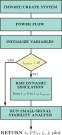
\includegraphics[width=0.35\linewidth]{inkscape_svg/block_diagram_full_code_smallsignal.pdf}
  \caption{Small-signal stability analysis full simulation block diagram. \textit{Source: Own elaboration.}}
  \label{fig:block_diagram_full_smallsignal}
\end{figure}

\begin{figure}[H]
  \centering
  \includegraphics[width=0.8\linewidth]{inkscape_svg/block_diagram_run_smallsignal.pdf}
  \caption{Small-signal stability analysis computation block diagram. \textit{Source: Own elaboration.}}
  \label{fig:block_diagram_run_smallsignal}
\end{figure}

\subsubsection{GUI implementation}

The GUI is creased using the open source program Qt Designer \cite{qt_designer}, which allows to create the GUI using a drag 
and drop interface. The GUI implementation consists on creating a new settings page for the small-signal stability analysis,
adding the option to run the simulation in the main tools bar, and creating a new results page to show the results of the simulation. 
The GUI implementationis not only adding the new pages, but also connecting the GUI with the code developed in Python.

However, the first initial step is to choose an icon for the small-signal stability analysis that will be shown in the tools bar and will 
hels users identify the option. The icon chosen is shown in Figure \ref{fig:small_signal_icon}. The icon represents a magnifying glass 
looking at a wave. The magnifying glass represents the small-signal analysis, which works around a small perturbation and a small interval
around the operating point, so the user needs the magnifying glass to see those small perturbations. The wave represents the system variables
represented in the time domain, which are the ones that will be analysed in the small-signal stability analysis.

\begin{figure}[H]
  \centering
  \includegraphics[width=0.25\linewidth]{inkscape_svg/small_signal_icon.pdf}
  \caption{Icon for the small-signal stability analysis. \textit{Source: VeraGrid \cite{veragrid}.}}
  \label{fig:small_signal_icon}
\end{figure}

The settings page shown in Figure \ref{fig:smallsignal_settings_GUI} allows the user to set the parameters needed for the small-signal stability analysis.
It is noted how the small-signal settings are added into the dynamic simulation settings. The settings shown are explained in the list below.

\begin{enumerate}
  \item \textit{Integration method}: The integration method to use if the RMS dynamic simulation is performed. There are two options: trapezoidal or implicit euler.
  \item \textit{Tolerance}: per-unit error tolerance to use in the integration method. Only needed if the Rms dynamic simulation is performed.
  \item \textit{Assessment time (s)}: The time instant in seconds where the stability assessment is performed.
  \item \textit{Time step (s)}: Step size in seconds between each numerical evaluation in the integration method. 
  Smaller intervals increase accuracy but require more computation. Only needed if the RMS dynamic simulation is performed.
\end{enumerate}


\begin{figure}[H]
  \centering
  \includegraphics[width=0.8\linewidth]{figures/settings_GUI.png}
  \caption{Small-signal stability analysis settings page. \textit{Source: VeraGrid \cite{veragrid}.}}
  \label{fig:smallsignal_settings_GUI}
\end{figure}

Figure \ref{fig:model_powerflow_GUI} shows the model page with the power flow already computed. The small-signal stability analysis can 
only be performed if the power flow has been computed, as it is needed to obtain the operating point of the system.

\begin{figure}[H]
  \centering
  \includegraphics[width=0.8\linewidth]{figures/model_powerflow_GUI.png}
  \caption{Model page with power flow already computed. \textit{Source: VeraGrid \cite{veragrid}.}}
  \label{fig:model_powerflow_GUI}
\end{figure}

\begin{figure}[H]
  \centering
  \begin{minipage}{0.45\textwidth}
    \centering
    \includegraphics[width=0.5\linewidth]{figures/results_desplegable_GUI.png}
    \caption{Results drowdown. \textit{Source: VeraGrid \cite{veragrid}.}}
    \label{fig:results_dropdown_GUI}
  \end{minipage}
  \hfill
  \begin{minipage}{0.5\textwidth}
    The results page shows the results of all the simulations performed in VeraGrid. The user can choose the results to show
    using the dropdown menu shown in Figure \ref{fig:results_dropdown_GUI}. In this case, the power flow and small-signal stability
     analysis results are shown. As one can see, the small-signal results are divided into 4 options: the modes table, the participation
     factors table, the complex domain plot and the complex domain plot in Hz. These results are shown in Figures \ref{fig:table_modes_GUI},
     \ref{fig:table_PF_GUI}, \ref{fig:plot_ss_GUI} and \ref{fig:plot_ss_Hz_GUI} respectively.
  \end{minipage}
\end{figure}

\begin{figure}[H]
  \centering
  \includegraphics[width=0.8\linewidth]{figures/result_modes_ss_GUI.png}
  \caption{Table result with the modes, damping ratio and oscillation frequencies. \textit{Source: VeraGrid \cite{veragrid}.}}
  \label{fig:table_modes_GUI}
\end{figure}

\begin{figure}[H]
  \centering
  \includegraphics[width=1\linewidth]{figures/result_pfactors_GUI.png}
  \caption{Table result with the participation factors. \textit{Source: VeraGrid \cite{veragrid}.}}
  \label{fig:table_PF_GUI}
\end{figure}

\begin{figure}[H]
  \centering
  \begin{minipage}{0.49\textwidth}
    \centering
    \includegraphics[width=\linewidth]{figures/smallsignal_plot_GUI.pdf}
    \caption{Complex domain plot.  \textit{Source: VeraGrid \cite{veragrid}.}}
    \label{fig:plot_ss_GUI}
  \end{minipage}
  \hfill
  \begin{minipage}{0.49\textwidth}
    \centering
    \includegraphics[width=\linewidth]{figures/smallsignal_plot_Hz_GUI.pdf}
    \caption{Complex domain plot in Hz. \textit{Source: VeraGrid \cite{veragrid}.}}
    \label{fig:plot_ss_Hz_GUI}
  \end{minipage}
\end{figure}

Figure \ref{fig:plot_ss_GUI} shows how the user can take a look at the eigenvalues exact values
by hovering the mouse over the points. Moreover, the 5\% damping ratio line is shown to help the user identify
the unstable modes. 









\subsection{Benchmark and validation}
\subsubsection{ANDES}

\subsubsection{Test case: Kundur two-area system}

The Kundur two-area system is a standard benchmark network widely used for small-signal and transient stability studies. It was introduced in the P. Kundur power system stability literature as a compact, yet representative, test case that exposes inter-area oscillatory modes and control interactions without excessive model complexity.

\begin{figure}[h!]
    \centering
    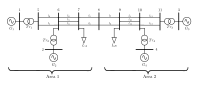
\includegraphics[width=1\linewidth]{figures/Kundur_system_no_shunt.pdf}
    \caption{Kundur two area system without shunt.}
    \label{fig:kundur_system}
\end{figure}

The main characteristics of the system, depicted in Figure \ref{fig:kundur_system}, are:
\begin{itemize}
    \item Two areas connected by a pair of parallel lines. In each area, 2 synchronous generators are placed so that each area can swing against each other and produce inter-area oscillations.
    \item All the synchronous generators are connected to the network through a transformer.
    \item In this version of the Kundur two-area system no shunts are connected to buses 7 and 9.
    \item The base power is 100 MW and the voltage levels are 20kV for the generators and 230kV for the network.
\end{itemize}

The following code can be used to model the Kundur two area system without shunt in VeraGrid and to perform the small-signal Stability analysis. As seen in the code, an event is created at time instant 2.5s where the active power of load A is increased to 900MW.
\newpage

\section{EMT Dynamic framework}\label{Chap2}
\input{Chapters/2_1TheoryEMT.tex}
\newpage

\section{Environmental, Social, and Gender Impact}
The present chapter considers the impact that this project has in the society.



\newpage

\cleardoublepage
\section{Budget}

TO CHECK!!!

The complete costs are detailed in Table~\ref{tab:equip}.

-	Les hores emprades per la realització del treball (les corresponents als crèdits del TFE). Millor 
si estan separades per les tasques executades segons la planificació. En una primera aproximació podeu considerar
 que una de les vostres hores es paga a 15 €/h.
-	Les despeses operatives: electricitat, calefacció, aigua o telefonia. Sumeu la part proporcional dels termes fixos.
 També tingueu en compte els viatges, les despeses d'oficina i d'altres.
-	Les despeses experimentals: materials, aigua, electricitat, combustibles, llicències, llibres.
-	Si és el cas, amortització dels equips. Considereu que un PC s'amortitza linealment en 5 anys i un telèfon mòbil en 3 anys.
-	Serveis abonats per obtenir algunes dades (per exemple d'un servei de microscòpia electrònica, encara que no ho hagi pagat l'estudiant).
-	I totes aquelles que haurien de constar si el treball fos realista i s'hagués de facturar. 


\begin{table}[!htb]\centering
	\caption{Total Costs.}
	\begin{tabular}{ccc|c}
		\hline
		\textbf{Concept} & \textbf{Unit cost (\texteuro/h)} & \textbf{Quantity (h)} & \textbf{Total (\texteuro)} \\
		\hline
		\hline
		Development engineer & 25.00 & 1,040 & 26,000.00 \\ 
		Supervisor & 30.00 & 260 & 7,800.00 \\
		\hline
		\textbf{Total} & & & 33,800.00 \\
		\hline
	\end{tabular}
	\label{tab:equip}
\end{table}




\cleardoublepage
\section{Time Planning}
Figure \ref{fig:gantt} shows the temporal evolution of the various tasks that have constituted the project.
\begin{figure}[H]
  \centering
  \resizebox{\textwidth}{!}{
  
  \begin{ganttchart}[y unit title=0.6cm,
  y unit chart=0.7cm,
  vgrid,hgrid, 
  title label anchor/.style={below=-1.6ex},
  title left shift=.05,
  title right shift=-.05,
  title height=1,
  progress label text={},
  bar height=0.5,
  group right shift=0,
  group top shift=.6,
  group height=.4]{1}{26}
  %labels
  \gantttitle{2025}{17} 
  \gantttitle{2026}{9}\\
  \gantttitle{September}{4} 
  \gantttitle{October}{5} 
  \gantttitle{November}{4} 
  \gantttitle{December}{4} 
  \gantttitle{January}{5} 
  \gantttitle{February}{4} \\
  %tasks
  \ganttbar[bar/.append style={fill=gray!60}]{\textbf{RMS Small-signal stability}}{1}{5} \\
  \ganttbar{Literature review}{1}{1} \\
  \ganttbar{Model development}{1}{1} \\
  \ganttbar{Benchmarking}{2}{3} \\
  \ganttbar{VeraGrid GUI integration}{4}{4} \\
  \ganttbar{Documentation}{5}{5} \\
  
  %relations 
  \ganttlink{elem1}{elem3} 
  \ganttlink{elem2}{elem3} 
  \ganttlink{elem3}{elem4} 
  \ganttlink{elem4}{elem5}
  \ganttlink{elem2}{elem5} 
  %\ganttlink{elem3}{elem4} 
  %\ganttlink{elem4}{elem5} 
  %\ganttlink{elem5}{elem6} 
  \end{ganttchart}
}
  \caption{Gantt Chart of the project.}
  \label{fig:gantt}
\end{figure}


\section{Conclusion}\label{Conclusion}

\subsection{Further Work}

The solver holds a lot of potential for enhancement, with many possible improvements of the existing features as well as future additions of new functionalities. Some of the 
future works that are being discussed are the following:

\begin{itemize}
    \item Related to raw performance, some intermediate calculations for the gradients and Hessians could be optimized to reduce the time needed to solve the problem. This involves using the sparse structures 
    used in the process of creating the Jacobian and Hessian matrices, although it is not a trivial task and requires a deep understanding of the data structure involved.


\end{itemize}
\newpage

\section*{Acknowledgments}\label{acknow} 
\addcontentsline{toc}{section}{Acknowledgments}
I want to thank Marc Cheah and Josep Fanals, my thesis supervisors from UPC and eRoots respectively, for the opportunity to develop this project in collaboration with Redeia and for their guidance and support through the process.
I'd also like to thank Santiago Peñate for his help in developing the tool and integrating it in GridCal in collaboration with Josep and me.

\appendix
\cleardoublepage

%bibliography
\cleardoublepage
%\renewcommand\refname{Bibliography}
%pdf\addcontentsline{toc}{section}{Bibliography}
\printbibliography
\end{document}

